\documentclass[11pt]{article}

\usepackage{report}

\usepackage[utf8]{inputenc}
\usepackage[T1]{fontenc}
\usepackage[colorlinks=true, linkcolor=black, citecolor=blue, urlcolor=blue]{hyperref}
\usepackage{url}
\usepackage{booktabs}
\usepackage{amsfonts}
\usepackage{amsmath}
\usepackage{nicefrac}
\usepackage{microtype}
\usepackage{graphicx}
\usepackage{natbib}
\usepackage{doi}
\usepackage{minted}
\usepackage{subfig}
\setcitestyle{aysep={,}}



\title{Predicting Food Groups \\ \vspace{0.5em} \large from nutritional information}

\author{
    David Sha\\
\AND
    Victoria Lyngaae\\
\AND
    Mason Sebek\\
\AND
    William Spongberg\\
\AND
\AND
	COMP20008: Elements of Data Processing\\
\AND
	The University of Melbourne\\
}

\date{May 2023}

\renewcommand{\headeright}{Predicting Food Groups from Nutritional Information}
\renewcommand{\undertitle}{Report}
\renewcommand{\shorttitle}{}

\begin{document}
\maketitle

\newpage
\tableofcontents
\thispagestyle{empty}

\newpage
\setcounter{page}{1}
\section{Introduction}

The objective of this project is to wrangle and analyse data contained within the \cite{FoodStandardsAustraliaNewZealand} dataset, for the purpose of answering an explicit and defined research question. We propose the inquiry: Can we predict the food group of a food item, based solely on its nutritional information? We implemented the supervised learning model of k-nearest-neighbours to predict and explore the relationship between nutritional information and food group classification.

\subsection{Research Question}
% 1. What is the research question?
To what extent can we predict the food group of a food item based solely on its nutritional information?

\subsection{Target Audience}
% 2. Who are the target audience.
The outcome of this project may be interesting to supermarket chains. If the model is sufficiently accurate, it could be used to detect food items that may not be labelled correctly or are missing labels. Better classification of food items can improve a supermarket's inventory management and/or product placement and ultimately improve the shopping experience of customers.

The findings of this exploration may be of value to a number of audiences, such as nutritionists, health researchers, consumers, educational institutions and food retailers.  An effective food group classification model has many practical applications such as:
\begin{itemize}
    \item Detection of food items that are labelled incorrectly, either by accident or with the intent to mislead consumers
    \item Improving a retailer's inventory management and product placement, and ultimately a customer's shopping experience
    \item Effective assessment of an individual's nutritional intake and dietary pattern
    \item Educating and enhancing public understanding of food groups, and general nutritional literacy
\end{itemize}



\subsection{Dataset}
% 3. The dataset you have chosen.
We make use of the dataset from \cite{FoodStandardsAustraliaNewZealand} containing 1616 food items and their nutritional information. This dataset contains all the information we need to answer our research question as each food item has a \verb|Classification| (food group) and respective nutritional information (such as energy, protein, etc.). To give us more context to the \verb|Classification| column, we also use a complementary dataset from \cite{FoodClassification} which maps numerical classifications to their respective food groups which become very useful when preprocessing the data and analysing the results.

\section{Methodology}

\emph{What wrangling and analysis methods (including at least one supervised learning method) have you applied? Why have you chosen these methods over other alternatives? How do you perform the experiment?}

\subsection{Data Wrangling}

\subsubsection{Preprocessing}

Prior to any use of machine learning, we evaluated  the quality of the data and found that it was not clean. Thus, we implemented various preprocessing techniques to ensure that the data was suitable to be included in the data pipeline. 


A large number of food items were wholly missing particular nutrition values. Understanding that this is likely an indication that a food has either an absence of the nutrient (eg, 0g) or that the food has not been checked for the nutrient's presence, we chose to set all NaN values to 0. Next, given that Food Standards Australia New Zealand (2013) indicates that the first two digits of a food's 'Classification' denote its major food group, each item's classification was simplified to these two characters. Given that there are 24 unique food groups (including unclassified items as a group), (Fig. 1) we also chose to simplify and compress less populated food groups, i.e., those containing very few food items, into a broader group, named miscellaneous. 

\begin{figure}[htbp]
    \centering
    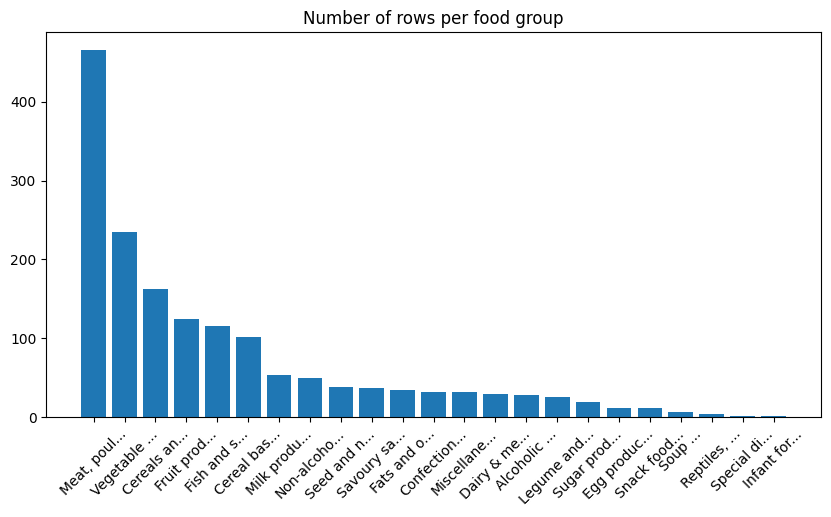
\includegraphics[width=0.9\textwidth]{report/figs/number-of-rows-per-food-group.png}
    \caption{The distribution of food items in twenty-three unique food groups in the \cite{FoodStandardsAustraliaNewZealand} dataset.}
    \label{fig:food-group-distribution}
\end{figure}

However, rather than arbitrarily choosing a number of food groups to be condensed into 'miscellaneous' (group 31), we opted to explore 3 different versions of the miscellaneous grouping; with 18, 10, and 2 groups (including the existing miscellaneous group) respectively condensed into miscellaneous. This can also be understood as providing the machine learning model with 6, 13 and 23 total labels, respectively for each variation.

\subsection{Data Analysis}
\subsubsection{Feature selection}

We also utilised the \verb|mutual_info_classif| from \verb|sklearn|'s feature selection module to evaluate which nutritional features contained the most useful information for classification. With each food item having up to 290 different nutritional measures, the data is highly dimensional, and thus, via feature selection, we improve the efficiency and effectiveness of the KNN model. We initially considered using a linear regression model, but opted to continue our investigation using k-NN, as this task called for classification, rather than determining the relationship between nutritional data. With the mutual information calculated, by choosing an appropriate threshold, we could remove some features that were not particularly insightful. This was done for each set of food groups, to ensure that they could be compared at their optimal performance each. 

\subsection{Supervised Learning}

\subsubsection{Training and test split}

With our data preprocessed and cleaned, we decided to use an 85\% training,15\% test split.  The model was created using only the \verb|train| data, to ensure that the model could be fairly tested and evaluated based on its performance on unseen data, thus avoiding overfitting and ensuring generalisation. 

We also employed a 10-fold cross validation approach to determine the optimal value of k for each set of food groups. Calculating the mean accuracy of the cross validated KNN model for a wide range of k values revealed that a k of 1 performed best for each variation, with measured mean accuracy ranging from 82.81\% to 89.15\%. Given that a k value of 1 may potentially cause the model to be overfitted it was decided to err on the side of caution and opt for each variation's next best k, especially given this is not wholly detrimental to the model's accuracy. 

\begin{figure}[htbp]
    \centering
    \subfloat[\centering 6 food groups]{{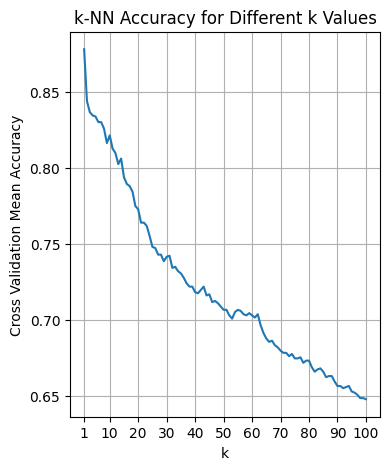
\includegraphics[height=5cm]{report/figs/knn-cross-validation-first.png} }}
    \qquad
    \subfloat[\centering 14 food groups]{{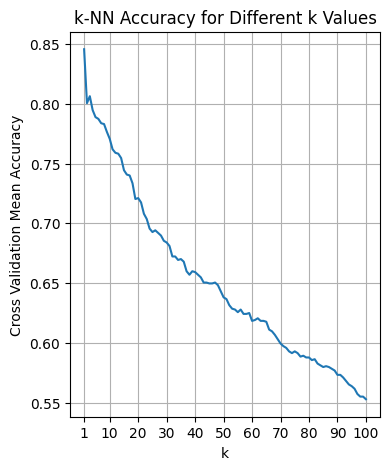
\includegraphics[height=5cm]{report/figs/knn-cross-validation-second.png} }}
    \qquad
    \subfloat[\centering 23 food groups]{{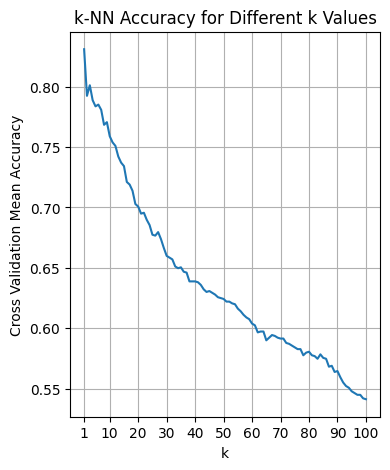
\includegraphics[height=5cm]{report/figs/knn-cross-validation-third.png} }}
    \caption{The $k$-nn cross validation mean accuracy for the 6, 14 and 23 food group classification models.}
    \label{fig:knn-cross-validation}
\end{figure}

Continuing with each variation’s optimal, we also evaluated the final knn model using cross validation. By splitting the test data into 7 folds, (to somewhat emulate the 85\% to 15\% training and test split), we were able to evaluate whether our model could consistently and accurately predict a food item’s food group, even when trained and tested on different sections of the preprocessed data; i.e., verify that the initial success of the model was not a fluke.

\section{Results}
\emph{What are the key results your research has obtained?}

\SaveVerb{topx}|TOP_X|
\begin{figure}[htbp]
    \centering
    \subfloat[\centering 6 food groups]{{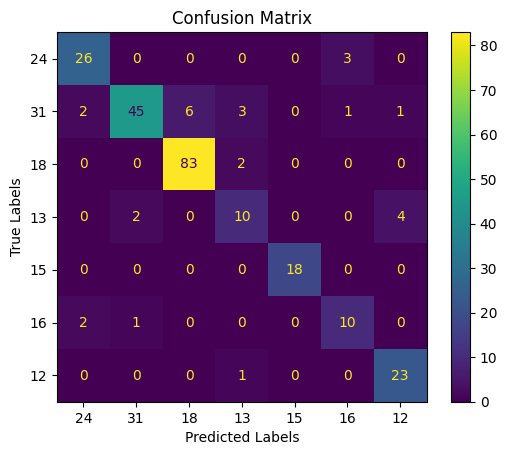
\includegraphics[height=6cm]{report/figs/knn-confusion-matrix-first.png} }}
    \qquad
    \subfloat[\centering 14 food groups]{{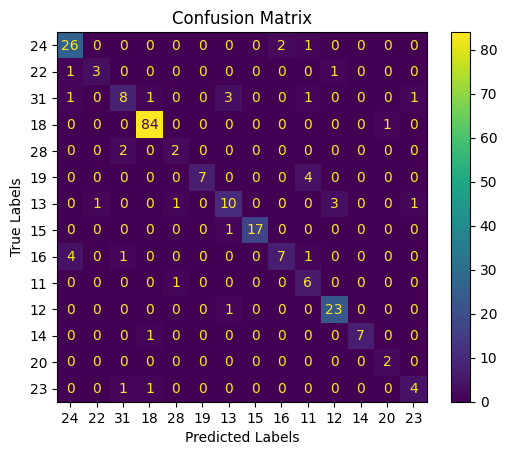
\includegraphics[height=6cm]{report/figs/knn-confusion-matrix-second.png} }}
    \qquad
    \subfloat[\centering 23 food groups]{{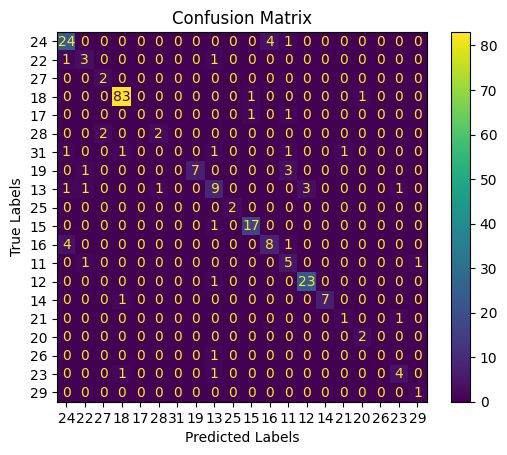
\includegraphics[height=6cm]{report/figs/knn-confusion-matrix-third.png} }}
    \caption{The confusion matrices for the \protect\UseVerb{topx} food group models.}
    \label{fig:confusion-matrices}
\end{figure}

% OUTDATED
In our analysis, we managed to achieve an accuracy score of 90.12\% (maybe not accurate?). Quite a high accuracy score suggests that our model can very accurately predict the classification of a food given its nutritional information. It is critical to note that during our evaluation process using 10-fold cross-validation, we witnessed a steep drop in our accuracy metrics, seeing accuracy range from 21.67\% to 65.94\%.
\section{Discussion}
\emph{Why are your results significant and valuable?}

Given our results have shown that our machine learning model has achieved an accuracy score of 90.12\%, it suggests that our model can very accurately predict the classification of a good given its nutritional information.(Add bit discussing benefits this can imply for use, specifically regarding our research question).

Interpretation of the results (What are the key results your research has obtained? Why are your results significant and valuable?)
Limitations and future improvements

DISCUSSION POINTS (not exhaustive):
3 variations of the span of miscellaneous group - elaborate on why we chose to do this (because it explores how preprocessing decisions affects the model etc, and because it shows the relationship between nutritional values and food groups and because some groups have few food items, elaborate more than this

Discuss what is shown in the graphs, compare the results of the three variations

If bootstrap accuracies is still much higher than cross validation and initial accuracy values, speculate why this has happened, research and refer to chatgpt screenshot on discord to help explain this
Refer back to what people understand to be a food group, what the outcome of this investigation tells us at the end of the day, elaborate on the significance and justification of the results

Interpret the results: WHAT DO THEY TELL US

Important - discuss thoroughly the limitations of the model, REFER TO RUBRIC FOR POINTS TO COVER


\section{Conclusion}
\emph{What are the limitations of your results and how can the project be improved for future?}

Throughout this investigation, we gained valuable insights into the data processing pipeline. The processes and strategies we utilised in preprocessing and analysis of the data elucidate the relationship between nutritional values and food groupings. With the ultimate goal of exploring and answering the question of ‘to what extent can we predict the food group of a food item based solely on its nutritional information?’,  this research endeavour has demonstrated this is entirely possible to achieve. It has also shown that the effectiveness of this enterprise is dependent on not only the initial data available, but also highly contingent on early-stages data cleaning and preparation. The validation and evaluation we conducted on our knn models supportively indicate that this is generally a successful way of predicting food groups, despite the aforementioned limitations. Future investigations of similar nature would tremendously benefit from use of a more well-rounded and balanced data set, given that some classifications in this data set have as few as one or two food items. With a much larger dataset, future experiments could also aim to classify sub-groups, i.e., minor food groups, rather than major.


\newpage
\bibliographystyle{plainnat}
\bibliography{references}


\end{document}
